\documentclass{article}
\usepackage{amsmath,amsthm,amssymb,amsfonts}
\usepackage{setspace,enumitem}
\usepackage{graphicx}
\usepackage{hyperref}
\usepackage{natbib}
\usepackage{afterpage}
\usepackage{xcolor}
\usepackage{etoolbox}
\usepackage{booktabs}
\usepackage{pdfpages}
\usepackage{multicol}
\usepackage{geometry}
\usepackage{accents}
\usepackage{bbm}
\usepackage{placeins}
\usepackage{verbatim}
\hypersetup{
	colorlinks,
	linkcolor={blue!90!black},
	citecolor={red!90!black},
	urlcolor={blue!90!black}
}

\newtheorem{theorem}{Theorem}
\newtheorem{assumption}{Assumption}
\newtheorem{definition}{Definition}
\newtheorem{lemma}{Lemma}
\setlength{\parindent}{0cm}
\geometry{margin = 1in}

\newcommand{\R}{\mathbb{R}}
\newcommand{\ubar}[1]{\underaccent{\bar}{#1}}
\newcommand{\Int}{\text{Int}}
\newcommand{\xbf}{\mathbf{x}}
\newcommand{\Abf}{\mathbf{A}}
\newcommand{\Bbf}{\mathbf{B}}
\newcommand{\Gbf}{\mathbf{G}}
\newcommand{\bbf}{\mathbf{b}}
\newcommand{\one}{\mathbbm{1}}

\newtoggle{extended}
\settoggle{extended}{false}

\title{FIN 970: Homework 2}
\author{Alex von Hafften }

\begin{document}

\maketitle

%%%%%%%%%%%%%%%%%%%%%%%%%%%%%%%%%%%%%%%%%%%%%%%%%%%%%%%%%%%%%%%%%%%%%%%%%%%%%%%%%%%%%%%%%%%%%%%%%%%%
%%%%%%%%%%%%%%%%%%%%%%%%%%%%%%%%%%%%%%%%%%%%%%%%%%%%%%%%%%%%%%%%%%%%%%%%%%%%%%%%%%%%%%%%%%%%%%%%%%%%
%%%%%%%%%%%%%%%%%%%%%%%%%%%%%%%%%%%%%%%%%%%%%%%%%%%%%%%%%%%%%%%%%%%%%%%%%%%%%%%%%%%%%%%%%%%%%%%%%%%%

\section{Cash-Flow and Return Predictability}

The goal for this exercise is to examine the evidence on cash flow and return predictability in the data.

\bigskip

Get annual data from 1930 to most recent period for log nominal market return $r_{d,t}^{\$}$, nominal dividends $\Delta d_{t}^{\$}$, and log price-dividend ratio $pd_t$ from CRSP. We also want to use log inflation rate $\pi_t$ (for example, from FRED) to help us convert nominal series into real.

\begin{enumerate}

\item To get real market returns, we can just subtract inflation from nominal market returns: $r_{d,t} = r^{\$}_{d,t} - \pi_t$. Do similar adjustment to remove inflation from nominal dividends.

\bigskip

\underline{Solution:} See \texttt{data.xlsx}.

\bigskip

\item Let us consider $h$-horizon forecasts of future cumulative returns and dividends:

\begin{align*}
\frac{1}{h} \sum_{j=1}^h \Delta d_{t+j} &= const + \beta_d x_t + error \\
\frac{1}{h} \sum_{j=1}^h \Delta r_{t+j} &= const + \beta_r x_t + error
\end{align*}

where $x_t$ is a predictive variable, and $h$ is the forecast horizon. We can compute slope coefficients and $R^2$ using standard OLS regressions.  Note the overlapping observations on the LHS - how would that affect the computation of the standard errors?

\bigskip

\underline{Solution:} Since we're average future dividends and returns, the observations on LHS are now mechanically correlated we each other.  For example, if $h=3$, the dividends in 1980 are included in the LHS variable for 1977, 1978, and 1979.  Asymptotic standard errors are only valid if observations are a random sample. Not accounting for this correlation will bias the standard errors upward.  For valid standard errors, we use bootstrap or use Newey-West standard errors.

\pagebreak

\item Run these regressions for the horizons of $h$ 1 year to 5 years, using price dividend ratio as a predictive variable, i.e. set $x_t = pd_t$. What are the slope coefficients and $R^2$s? Do you find the signs of slope coefficients reasonable? What is the statistical significance of the slope coefficients and the $R^2$s? What does this evidence suggest in terms of the drivers of the aggregate equity prices in the data?

\bigskip

\underline{Solution:} My estimates for slope coefficients and $R^2$s are within the confidence intervals for such regression in the lecture slides.  My regressions feature the same pattern for dividends the $R^2$s starts relatively high and then drops as you extend the forecasting window and the $R^2$s for returns starts relatively low and increases. The significance and magnitude of the slope coefficients for the dividend regressions grow whereas the slope coefficient for the return regressions stay about the same magnitude and become more significant. For dividend, the sign of the slope coefficients indicate that higher $pd$ ratios predict higher future dividends and lower market returns.  This suggests that $pd$ ratios are better predictors of returns than dividends.

\bigskip


% Table created by stargazer v.5.2.3 by Marek Hlavac, Social Policy Institute. E-mail: marek.hlavac at gmail.com
% Date and time: Mon, Mar 28, 2022 - 21:55:38
\begin{table}[!htbp] \centering 
  \caption{Dividends} 
  \label{} 
\begin{tabular}{@{\extracolsep{5pt}}lccccc} 
\\[-1.8ex]\hline 
\hline \\[-1.8ex] 
 & \multicolumn{5}{c}{\textit{Dependent variable:}} \\ 
\cline{2-6} 
\\[-1.8ex] & delta\_d\_1 & delta\_d\_2 & delta\_d\_3 & delta\_d\_4 & delta\_d\_5 \\ 
\\[-1.8ex] & (1) & (2) & (3) & (4) & (5)\\ 
\hline \\[-1.8ex] 
 pd & 0.077$^{***}$ & 0.055$^{***}$ & 0.039$^{***}$ & 0.029$^{**}$ & 0.024$^{**}$ \\ 
  & (0.024) & (0.019) & (0.015) & (0.011) & (0.009) \\ 
  & & & & & \\ 
 Constant & $-$0.246$^{***}$ & $-$0.169$^{**}$ & $-$0.115$^{**}$ & $-$0.077$^{*}$ & $-$0.058$^{*}$ \\ 
  & (0.084) & (0.067) & (0.052) & (0.039) & (0.031) \\ 
  & & & & & \\ 
\hline \\[-1.8ex] 
Observations & 91 & 90 & 89 & 88 & 87 \\ 
R$^{2}$ & 0.100 & 0.083 & 0.074 & 0.071 & 0.074 \\ 
\hline 
\hline \\[-1.8ex] 
\textit{Note:}  & \multicolumn{5}{r}{$^{*}$p$<$0.1; $^{**}$p$<$0.05; $^{***}$p$<$0.01} \\ 
\end{tabular} 
\end{table} 


% Table created by stargazer v.5.2.3 by Marek Hlavac, Social Policy Institute. E-mail: marek.hlavac at gmail.com
% Date and time: Tue, Mar 22, 2022 - 16:31:05
\begin{table}[!htbp] \centering 
  \caption{Market Returns} 
  \label{} 
\begin{tabular}{@{\extracolsep{5pt}}lccccc} 
\\[-1.8ex]\hline 
\hline \\[-1.8ex] 
 & \multicolumn{5}{c}{\textit{Dependent variable:}} \\ 
\cline{2-6} 
\\[-1.8ex] & r\_1 & r\_2 & r\_3 & r\_4 & r\_5 \\ 
\\[-1.8ex] & (1) & (2) & (3) & (4) & (5)\\ 
\hline \\[-1.8ex] 
 pd & $-$0.054 & $-$0.068$^{**}$ & $-$0.061$^{***}$ & $-$0.058$^{***}$ & $-$0.057$^{***}$ \\ 
  & (0.043) & (0.028) & (0.020) & (0.017) & (0.015) \\ 
  & & & & & \\ 
 Constant & 0.252$^{*}$ & 0.302$^{***}$ & 0.279$^{***}$ & 0.267$^{***}$ & 0.266$^{***}$ \\ 
  & (0.148) & (0.098) & (0.070) & (0.058) & (0.051) \\ 
  & & & & & \\ 
\hline \\[-1.8ex] 
Observations & 91 & 90 & 89 & 88 & 87 \\ 
R$^{2}$ & 0.017 & 0.061 & 0.092 & 0.119 & 0.151 \\ 
\hline 
\hline \\[-1.8ex] 
\textit{Note:}  & \multicolumn{5}{r}{$^{*}$p$<$0.1; $^{**}$p$<$0.05; $^{***}$p$<$0.01} \\ 
\end{tabular} 
\end{table} 


\end{enumerate}

See \texttt{data.R} for regressions.

\pagebreak

%%%%%%%%%%%%%%%%%%%%%%%%%%%%%%%%%%%%%%%%%%%%%%%%%%%%%%%%%%%%%%%%%%%%%%%%%%%%%%%%%%%%%%%%%%%%%%%%%%%%
%%%%%%%%%%%%%%%%%%%%%%%%%%%%%%%%%%%%%%%%%%%%%%%%%%%%%%%%%%%%%%%%%%%%%%%%%%%%%%%%%%%%%%%%%%%%%%%%%%%%
%%%%%%%%%%%%%%%%%%%%%%%%%%%%%%%%%%%%%%%%%%%%%%%%%%%%%%%%%%%%%%%%%%%%%%%%%%%%%%%%%%%%%%%%%%%%%%%%%%%%

\section{Twist on Log-Linearization}

The return log-linearization formula is typically written as

\begin{align}
r_{t+1} \approx \kappa_0 + \kappa_1 pd_{t+1} - pd_t + \Delta d_{t+1} \label{p3_ll1}
\end{align}

where $\kappa_0$ and $\kappa_1$ are log-linearization constants which depend on the mean of price-dividend ratio. Use their solution to show that you can rewrite this formula in the following way:

\begin{align}
r_{t+1} \approx - \log \kappa_1 + \kappa_1 \tilde{pd}_{t+1} - \tilde{pd}_t + \Delta d_{t+1} \label{p3_ll2}
\end{align}

where $\tilde{pd}$ is the demeaned price-dividend ratio, $\tilde{pd}_t = pd_t - E(pd_t)$.  There is nothing deep about this result. However, it's oftentimes more convenient to use (e.g., in equilibrium model solutions), as we do not need to keep track of $\kappa_0$ and the (unimportant) intercepts in the solution of price-dividend ratios.

\bigskip

\underline{Solution:} Following the lecture notes from class,

\begin{align*}
R_{t+1} 
&= \frac{P_{t+1} + D_{t+1}}{P_t}\\
&= \frac{D_{t+1}(\frac{P_{t+1}}{D_{t+1}} + 1)}{D_t \frac{P_t}{D_t}}\\
&= \frac{D_{t+1}}{D_t} \frac{PD_{t+1} + 1}{PD_{t}}\\
\text{where } PD_t &:= P_t/D_t \\
\implies
\log(R_t) &= \log(\frac{D_{t+1}}{D_t}) + \log(PD_{t+1} + 1) - \log(PD_t)\\
r_t &= \Delta d_{t+1} - pd_t + \log(\exp(pd_t)+1)\\
\text{where } r_t &:= \log(R_t)\\
\text{and } pd_t &:= \log(PD_t)\\
f(x) &:= \log(\exp(x) + 1)\\
\implies
f'(x) &= \frac{\exp(x)}{\exp(x) + 1} \\
f(x) &\approx f(\bar{x}) + f'(\bar{x})(x - \bar{x}) \\ 
&= \log(\exp(\bar{x}) + 1) + \frac{\exp(\bar{x})}{\exp(\bar{x}) + 1}(x - \bar{x})\\
\implies
\log(\exp(pd_t)+1) &\approx \log(\exp(E(pd_t))+1) + \frac{\exp(E(pd_t))}{\exp(E(pd_t)) + 1}(pd_t - E(pd_t)) \\
\implies
r_{t+1} &\approx \Delta d_{t+1} - pd_t + \log(\exp(E(pd_t))+1) + \frac{\exp(E(pd_t))}{\exp(E(pd_t)) + 1}(pd_t - E(pd_t)) \\
&= \kappa_0 + \kappa_1 pd_{t+1} + \Delta d_{t+1} - pd_t \\
\text{where }
\kappa_0 &= \log(\exp(E(pd_t))+1) - \frac{\exp(E(pd_t))}{\exp(E(pd_t)) + 1}E(pd_t)\\
\text{and }
\kappa_1 &= \frac{\exp(E(pd_t))}{\exp(E(pd_t)) + 1}
\end{align*}

\pagebreak

($\ref{p3_ll1}$) and ($\ref{p3_ll2}$) are equivalent iff 

\begin{align*}
\kappa_0 + \kappa_1 pd_{t+1} - pd_t 
&= - \log k_1 + \kappa_1 \tilde{pd}_{t+1} - \tilde{pd}_t \\
\iff
\Bigg[\log(\exp(E(pd_t))+1) - \frac{\exp(E(pd_t))}{\exp(E(pd_t)) + 1}E(pd_t)\Bigg] &+ \Bigg[ \frac{\exp(E(pd_t))}{\exp(E(pd_t)) + 1} \Bigg] pd_{t+1} - pd_t \\
= - \log \Bigg[ \frac{\exp(E(pd_t))}{\exp(E(pd_t)) + 1} \Bigg] &+ \Bigg[ \frac{\exp(E(pd_t))}{\exp(E(pd_t)) + 1} \Bigg] [pd_{t+1} - E(pd_{t+1})] - [pd_{t} - E(pd_{t})] \\
\iff
\log(\exp(E(pd_t))+1) &- \frac{\exp(E(pd_t))}{\exp(E(pd_t)) + 1}E(pd_t)\\
= - \log \Bigg[ \frac{\exp(E(pd_t))}{\exp(E(pd_t)) + 1} \Bigg] -& \Bigg[ \frac{\exp(E(pd_t))}{\exp(E(pd_t)) + 1} \Bigg] E(pd_{t+1}) + E(pd_{t}) \\
\iff
\log(\exp(E(pd_t))+1) &- \frac{\exp(E(pd_t))}{\exp(E(pd_t)) + 1}E(pd_t)\\
= - \log (\exp(E(pd_t))) &+ \log(\exp(E(pd_t)) + 1) - \Bigg[ \frac{\exp(E(pd_t))}{\exp(E(pd_t)) + 1} \Bigg] E(pd_{t+1}) + E(pd_{t}) \\
\iff
- \frac{\exp(E(pd_t))}{\exp(E(pd_t)) + 1}E(pd_t)
&= - E(pd_t) - \Bigg[ \frac{\exp(E(pd_t))}{\exp(E(pd_t)) + 1} \Bigg] E(pd_{t+1}) + E(pd_{t}) \\
\iff
- \frac{\exp(E(pd_t))}{\exp(E(pd_t)) + 1}E(pd_t)
&= - \Bigg[ \frac{\exp(E(pd_t))}{\exp(E(pd_t)) + 1} \Bigg] E(pd_{t+1}) \\
E(pd_t)
&= E(pd_{t+1})
\end{align*}

$E(pd_t)= E(pd_{t+1})$ holds iff $pd_t$ is a martingale.

\pagebreak

%%%%%%%%%%%%%%%%%%%%%%%%%%%%%%%%%%%%%%%%%%%%%%%%%%%%%%%%%%%%%%%%%%%%%%%%%%%%%%%%%%%%%%%%%%%%%%%%%%%%
%%%%%%%%%%%%%%%%%%%%%%%%%%%%%%%%%%%%%%%%%%%%%%%%%%%%%%%%%%%%%%%%%%%%%%%%%%%%%%%%%%%%%%%%%%%%%%%%%%%%
%%%%%%%%%%%%%%%%%%%%%%%%%%%%%%%%%%%%%%%%%%%%%%%%%%%%%%%%%%%%%%%%%%%%%%%%%%%%%%%%%%%%%%%%%%%%%%%%%%%%

\section{External Habits}

Consider an environment very similar to the external habits model of Campbell-Cochrane, 1999.

\begin{itemize}

\item Investors have utility over consumption relative to a reference point $X_t$:

$$
u_t = \frac{(C_t - X_t)^{1-\gamma} - 1}{1-\gamma}
$$

\item Consumption growth is iid Normal:

$$
\Delta c_{t+1} = g + v_{t +1}, \;\;\; Var(v_{t+1}) = \sigma_v^2
$$

\item Define surplus consumption $S_t$:

$$
S_t = \frac{C_t - X_t}{C_t}
$$

\item Log surplus consumption is driven by the consumption news:

$$
s_{t+1} = \bar{s} + \phi(s_t - \bar{s}) + \lambda(s_t) v_{t+1}
$$

where the sensitivity function is specified as in CC, 99:

$$
\lambda(s) = \frac{1}{\bar{S}} \sqrt{1 - 2(s-\bar{s})} - 1,
$$

when $s_t < s_{max}$ and 0 otherwise.

\item The only difference between CC, 99 is the specification of $\bar{s} = \log \bar{S}$

$$
\bar{S} = \sigma_v \sqrt{\frac{\gamma}{1- \phi - b/\gamma}}
$$

where $b$ is a preference parameter.

\end{itemize}

\begin{enumerate}

\item Show that the one-period real risk-free rates are now time-varying, and are linear in the consumption surplus $s_t$.

\underline{Solution:} Manipulating consumption growth:

$$
\Delta c_{t+1} = g + v_{t +1} 
\implies 
\frac{C_{t+1}}{C_t} = \exp(g + v_{t+1})
$$

Manipulating the surplus consumption law of motion:

$$
s_{t+1} = \bar{s} + \phi(s_t - \bar{s}) + \lambda(s_t) v_{t+1} 
\implies 
\frac{S_{t+1}}{S_t} = \exp((\phi-1)(s_t - \bar{s}) + (1 + \lambda(s_t))v_{1+t})
$$

Plugging consumption surplus into the utility function:

$$
u_t = \frac{(C_t S_t)^{1-\gamma} - 1}{1-\gamma} \implies u_{c, t} = (C_t S_t)^{-\gamma}
$$

\pagebreak

Thus, the stochastic discount factor is:

\begin{align*}
M_{t+1} 
&= \beta \frac{u_{c, t+1}}{u_{c, t}} \\
&= \beta \frac{(C_{t+1} S_{t+1})^{-\gamma}}{(C_t S_t)^{-\gamma}} \\
&= \beta \Bigg(\frac{C_{t+1}}{C_t}\Bigg)^{-\gamma} \Bigg(\frac{S_{t+1}}{S_t}\Bigg)^{-\gamma} \\
&= \beta \exp(-\gamma(g + v_{t+1})) \exp(-\gamma[(\phi-1)(s_t - \bar{s}) + (1 + \lambda(s_t))v_{1+t})]) \\
&= \beta \exp(-\gamma g)\exp(\gamma(1-\phi)(s_t - \bar{s}))\exp(\underbrace{-\gamma(1+\lambda(s_t))v_{t+1}}_{\sim Normal(0, \gamma^2(1+\lambda(s_t))^2\sigma_v^2)})
\end{align*}

The expected value of the stochastic discount factor is

\begin{align*}
E_t[M_{t+1}]
&= E_t[\beta \exp(-\gamma g)\exp(\gamma(1-\phi)(s_t - \bar{s}))\exp(-\gamma(1+\lambda(s_t))v_{t+1})]\\
&= \beta \exp(-\gamma g)\exp(\gamma(1-\phi)(s_t - \bar{s}))E_t[\exp(-\gamma(1+\lambda(s_t))v_{t+1})]\\
&= \beta \exp(-\gamma g)\exp(\gamma(1-\phi)(s_t - \bar{s}))\exp\Bigg(\frac{1}{2}\gamma^2 (1+\lambda(s_t))^2\sigma_v^2\Bigg)
\end{align*}

using the MGF of the normal distribution (i.e., if $X \sim N(\mu, \sigma^2)$ then $E[\exp(tX)] = \exp(\mu t + \sigma^2 t^2/2)$).

The gross risk free rate is:

\begin{align*}
R^f_t 
&= \frac{1}{E_t[M_{t+1}]} \\
&= \frac{1}{\beta} \exp(\gamma g) \exp(-\gamma(1 - \phi)(s_t - \bar{s})) \exp\Bigg(-\frac{1}{2}\gamma^2 (1+\lambda(s_t))^2\sigma_v^2\Bigg)
\end{align*}

Taking logs,

\begin{align*}
r^f_t 
&= -\log(\beta) + \gamma g - \gamma(1 - \phi)(s_t - \bar{s}) - \frac{1}{2}\gamma^2 (1+\lambda(s_t))^2\sigma_v^2\\
&= -\log(\beta) + \gamma g - \gamma(1 - \phi)(s_t - \bar{s}) - \frac{1}{2}\gamma^2 \Bigg(\frac{1}{\bar{S}} \sqrt{1 - 2(s_t-\bar{s})}\Bigg)^2\sigma_v^2\\
&= -\log(\beta) + \gamma g - \gamma(1 - \phi)(s_t - \bar{s}) - \frac{1}{2}\gamma^2 \frac{1}{\Bigg(\sigma_v \sqrt{\frac{\gamma}{1- \phi - b/\gamma}}
\Bigg)^2} (1 - 2(s_t-\bar{s}))\sigma_v^2\\
&= -\log(\beta) + \gamma g - \gamma(1 - \phi)(s_t - \bar{s}) - \frac{1}{2}\gamma (1- \phi - b/\gamma)(1 - 2(s_t-\bar{s}))\\
&= -\log(\beta) + \gamma g - \gamma s_t + \gamma \bar{s} + \gamma \phi s_t - \gamma \phi \bar{s} - \frac{1}{2} (\gamma - \gamma \phi - b) + s_t \gamma - s_t \gamma \phi - s_t b - \bar{s} \gamma + \bar{s} \gamma \phi + \bar{s} b\\
&= -\log(\beta) + \gamma g  - \frac{1}{2} (\gamma - \gamma \phi - b)  -  b (s_t - \bar{s})
\end{align*}

by substituting in for $\lambda(s_t)$ and $\bar{S}$.  Clearly, $r^f_t$ is linear in $s_t$ and time varying through $s_t$.

\pagebreak

\item Consider the case of $b > 0$ - this is the case studied in Wachter, 2006. How do the interest rates vary with the consumption surplus ratio? Are they low or high in ``good times"? Are the real bonds risky in this model, or do they hedge aggregate risks?

\underline{Solution:} As discussed in Wachter (2006), if $b <0$, intertemporal smoothing dominates precautionary savings, so an increase in surplus consumptions drives down interest rates. Formally, $b > 0$, $\frac{\partial r^f_t }{\partial s_t} = -b < 0$. Interest rates are low for in times with high consumption surplus ratios. High consumption surpluses correspond to ``good times".

\bigskip

Consider any (possibly risky) bond with real return $R_{t+1}$. If the bond is traded, then the Euler equation must hold:

\begin{align*}
E_t[M_{t+1} R_{t+1}] &= 1\\
\implies
E_t[M_{t+1}] E_t[R_{t+1}] + Cov_t(M_{t+1}, R_{t+1})&= 1\\
\implies
E_t[R_{t+1}] + \frac{Cov_t(M_{t+1}, R_{t+1})}{E_t[M_{t+1}] }&= \frac{1}{E_t[M_{t+1}] }\\
\implies
E_t[R_{t+1}] + \frac{Cov_t(M_{t+1}, R_{t+1})}{E_t[M_{t+1}] }&= R^f_{t+1}\\
\implies
E_t[R_{t+1}] - R^f_{t+1} 
&= -\frac{Cov_t(M_{t+1}, R_{t+1})}{E_t[M_{t+1}] } \\
&= -\frac{\rho_t(M_{t+1}, R_{t+1}) \sigma_t(M_{t+1})\sigma_t(R_{t+1})}{E[M_{t+1}] } \\
\implies
\frac{E_t[R_{t+1}] - R^f_{t+1} }{\sigma_t(R_{t+1})}
&= - \rho_t(M_{t+1}, R_{t+1}) \frac{\sigma_t(M_{t+1}) }{E_t[M_{t+1}] } \\
&\approx - \rho_t(M_{t+1}, R_{t+1}) \gamma \sigma_v^2(1+\lambda(s_t))
\end{align*}

with the last approximation following from the log-normality of $M_{t+1}$ conditional on time-$t$ information (see Wachter 2006; still need to verify the logic on my own).  Since $\lambda(s_t)$ is decreasing in $s$, risk premia move counter-cyclically (i.e. risk premia are high when $s_t$ is low).  So yes, real bonds are risky and they do hedge aggregate risks because the expected excess returns are higher in ``bad times."

\item Compare the behavior of interest rates in this model with the predictions in the Long-Run Risk model.  In the long-run risks model, do real rates fall or rise in ``good" times (think about ``good" times as high expected growth and/or low conditional volatility).

\underline{Solution:}  In the Long-Run Risk model, the risk-free rate is

$$
r_{f,t} = -\log \delta + \frac{1}{\psi} (\mu + x_t) + r_\sigma \sigma_t^2
$$

(see Long-Run Risk question or lecture notes) where $\psi > 1$ is the intertemporal elasticity of substitution and $r_q < 0$ is the loading on the conditional volatility.  In the Long-Run risk model, the risk-free rate increases is good times (i.e. $x_t$ is high and $\sigma_t$ is low): $\frac{\partial r_{f,t}}{\partial x_t} = \frac{1}{\psi} > 0$ and $\frac{\partial r_{f,t}}{\partial \sigma_t} = r_q < 0$. 

\item Can you use these model predictions to test the two asset-pricing theories? How would you do that?

\underline{Solution:} Yes, we can look at good times (i.e., with high consumption growth and low volatility) and bad times (i.e., with low consumption growth and high volatility).  If interest rates are higher in good times, this evidence is supportive of the long-run risk models, but if interest rates are higher in bad times, this evidence is supportive of the habits models.

\end{enumerate}

\pagebreak

%%%%%%%%%%%%%%%%%%%%%%%%%%%%%%%%%%%%%%%%%%%%%%%%%%%%%%%%%%%%%%%%%%%%%%%%%%%%%%%%%%%%%%%%%%%%%%%%%%%%
%%%%%%%%%%%%%%%%%%%%%%%%%%%%%%%%%%%%%%%%%%%%%%%%%%%%%%%%%%%%%%%%%%%%%%%%%%%%%%%%%%%%%%%%%%%%%%%%%%%%
%%%%%%%%%%%%%%%%%%%%%%%%%%%%%%%%%%%%%%%%%%%%%%%%%%%%%%%%%%%%%%%%%%%%%%%%%%%%%%%%%%%%%%%%%%%%%%%%%%%%

\section{Long-Run Risks Model}

Consider the following specification of the long-run risks model. Consumption and dividend dynamics are given by

\begin{align*}
\Delta c_{t+1} &= \mu_g + x_t + \sigma_t \eta_{t+1}, \\
x_{t+1} &= \rho x_t + \varphi_e \sigma_t e_{t+1}, \\
\sigma_{t+1}^2 &= \sigma_0^2 + \nu(\sigma_t^2 - \sigma_0^2) + \sigma_w w_{t+1},\\
\Delta d_{t+1} &= \mu_d + \phi x_t + \pi_d \sigma_t \eta_{t+1} + \varphi_d \sigma_t u_{d,t+1}
\end{align*}

where all shocks are iid uncorrelated standard Normal.

\bigskip

The investor has recursive Epstein-Zin preferences over the future consumption,

$$
U_t = \Bigg[(1-\delta)C_t^{1- \frac{1}{\psi}} + \delta (E_t U_{t+1}^{1 - \gamma})^{\frac{1-\frac{1}{\psi}}{1 - \gamma}} \Bigg]^{\frac{1}{1-\frac{1}{\psi}}}
$$

Theoretical Model Solution

\begin{enumerate}

\item Conjecture that price-consumption ratio is linear in expected growth,

$$
pc_t = A_0 + A_x x_t + A_\sigma \sigma_t^2,
$$

and use Euler equation on consumption asset and log-linearization of consumption return to solve for $A_0,A_x,A_\sigma$ and log-linearization coefficient $\kappa_1$ in terms of the fundamental model parameters. Under what conditions asset valuations respond positively to expected growth? negatively to consumption volatility? What do those conditions mean, economically?

\bigskip

\underline{Solution:}  The stochastic discount factor for Epstein-Zin preferences (without labor income) is:

\begin{align*}
M_{t+1} 
&= \frac{U_{c,t+1}}{U_{c,t}}\\
&= \delta^{\theta}\Bigg(\frac{C_{t+1}}{C_t}\Bigg)^{-\frac{\theta}{\psi}} R_{C,t+1}^{\theta-1}
\end{align*}

where $R_{C,t+1} = \frac{W_{t+1}}{W_t - C_t}$ is the gross return on the aggregate consumption portfolio and $\theta \equiv \frac{1-\gamma}{1 - \frac{1}{\psi}}$.  Taking logs,

\begin{align*}
m_{t+1} 
&= \log M_{t+1}\\
&= \theta \log \delta - \frac{\theta}{\psi} \Delta c_{t+1} + (\theta - 1) r_{c,t+1}\\
\end{align*}

where $\Delta c_{t+1} = \log(C_{t+1}/C_t)$ and $r_{c,t+1} = \log R_{C,t+1}$.  

\pagebreak

Using the Campbell-Schiller approximation to log-linearization the consumption return:

\begin{align*}
R_{C,t+1} 
&= \frac{P_{C,t+1} + C_{t+1}}{P_{C,t}} \\
&=  \frac{\frac{P_{C,t+1}}{C_{t+1}} + 1}{\frac{P_{C,t}}{C_t}} \frac{C_{t+1}}{C_{t}}\\
r_{c,t+1} 
&= \log(\exp(pc_{t+1}) +1) - pc_t +\Delta c_{t+1} \\
&\approx \Bigg[\log(\exp(\bar{pc}) +1) + \frac{\exp(\bar{pc})}{\exp(\bar{pc}) + 1} (pc_{t+1} - \bar{pc})\Bigg]- pc_t +\Delta c_{t+1} \\
&= \underbrace{\log(\exp(\bar{pc}) +1)- \frac{\exp(\bar{pc})}{\exp(\bar{pc}) + 1} \bar{pc}}_{\equiv \kappa_0} + \underbrace{\frac{\exp(\bar{pc})}{\exp(\bar{pc}) + 1}}_{\equiv \kappa_1} pc_{t+1} - pc_t +\Delta c_{t+1} 
\end{align*}

where $pc_t = \log(P_{C,t}/C_{t})$. Using the result from problem 2,

\begin{align*}
r_{c, t+1} 
&= \kappa_0 + \kappa_1 pc_{t+1} - pc_t + \Delta c_{t+1}\\
&= -\log \kappa_1 + \kappa_1 \underbrace{\tilde{pc}_{t+1}}_{\equiv pc_{t+1} - \bar{pc}} - \tilde{pc}_t + \Delta c_{t+1}
\end{align*}

Given the guess for $pc_t$, its unconditional expected value is $\bar{pc} = A_0 + A_\sigma \sigma_0^2$, so $\tilde{pc}_t = A_x x_t + A_\sigma (\sigma_t^2 - \sigma_0^2)$.  Plugging the dynamics for volatility and consumption:

\begin{align*}
\tilde{pc}_{t+1} 
&= A_x x_{t+1} + A_\sigma (\sigma_{t+1}^2 - \sigma_0^2)\\
&= A_x [\rho x_t + \varphi_e \sigma_t e_{t+1}] + A_\sigma [\nu(\sigma_t^2 - \sigma_0^2) + \sigma_w w_{t+1}]\\
&= A_x \rho x_t + A_\sigma \nu(\sigma_t^2 - \sigma_0^2) + A_x \varphi_e \sigma_t e_{t+1}  + A_\sigma \sigma_w w_{t+1}
\end{align*}

Plugging into the consumption return:

\begin{align*}
r_{c, t+1} 
&= -\log \kappa_1 + \kappa_1 [A_x \rho x_t + A_\sigma \nu(\sigma_t^2 - \sigma_0^2) + A_x \varphi_e \sigma_t e_{t+1}  + A_\sigma \sigma_w w_{t+1}] \\&- [A_x x_t + A_\sigma (\sigma_t^2 - \sigma_0^2)] + [\mu_g + x_t + \sigma_t \eta_{t+1}]\\
&= [-\log \kappa_1 + \mu_g] + [\kappa_1 A_x \rho - A_x + 1] x_t
+ [\kappa_1 A_\sigma \nu - A_\sigma](\sigma_t^2 - \sigma_0^2) \\
&+ \kappa_1 A_x \varphi_e \sigma_t e_{t+1} 
+ \kappa_1 A_\sigma \sigma_w w_{t+1}
+ \sigma_t \eta_{t+1}
\end{align*}


For any asset with return $R_{i,t+1}$, the Euler equation holds and if the return is log-normal:

\begin{align*}
1 &= E_t[M_{t+1} R_{i,t+1}]\\
&= E_t[\exp(m_{t+1} + r_{i,t+1})]\\
&= \exp(E_t[m_{t+1} + r_{i,t+1}] + \frac{1}{2} Var_t[m_{t+1} + r_{i,t+1}])\\
\implies
0&= E_t[m_{t+1} + r_{i,t+1}] + \frac{1}{2} Var_t[m_{t+1} + r_{i,t+1}]
\end{align*}

\pagebreak

In particular for the consumption assets, the Euler equation holds. 

\begin{align*}
m_{t+1} + r_{c,t+1} 
&= \theta \log \delta - \frac{\theta}{\psi} \Delta c_{t+1} + \theta r_{c,t+1}\\
&=\theta \log \delta - \frac{\theta}{\psi} [\mu_g + x_t + \sigma_t \eta_{t+1}] \\
&+ \theta[-\log \kappa_1 + \mu_g] + 
\theta[\kappa_1 A_x \rho - A_x + 1] x_t
+ \theta[\kappa_1 A_\sigma \nu - A_\sigma](\sigma_t^2 - \sigma_0^2) \\
&+ \theta\kappa_1 A_x \varphi_e \sigma_t e_{t+1} 
+ \theta\kappa_1 A_\sigma \sigma_w w_{t+1}
+ \theta\sigma_t \eta_{t+1}\\
&=\theta \log \delta - \frac{\theta}{\psi} [\mu_g + x_t + \sigma_t \eta_{t+1}] \\
&+ \theta[-\log \kappa_1 + \mu_g] + 
\theta[\kappa_1 A_x \rho - A_x + 1] x_t
+ \theta[\kappa_1 A_\sigma \nu - A_\sigma](\sigma_t^2 - \sigma_0^2) \\
&+ \theta\kappa_1 A_x \varphi_e \sigma_t e_{t+1} 
+ \theta\kappa_1 A_\sigma \sigma_w w_{t+1}
+ \theta\sigma_t \eta_{t+1}\\
&= \theta[\log \delta - \log \kappa_1 + (1- \frac{1}{\psi})\mu_g ] + \theta[\kappa_1 A_x \rho - A_x + 1 - \frac{1}{\psi}] x_t \\
&+ \theta[\kappa_1 A_\sigma \nu - A_\sigma](\sigma_t^2 - \sigma_0^2) + \theta\kappa_1 A_x \varphi_e \sigma_t e_{t+1}  \\
&+ \theta\kappa_1 A_\sigma \sigma_w w_{t+1} + \theta (1-\frac{1}{\psi}) \sigma_t \eta_{t+1}
\end{align*}

The expected value and variance of $m_{t+1} + r_{c,t+1}$ is

\begin{align*}
E_t[m_{t+1} + r_{c,t+1}] 
&= \theta[\log \delta - \log \kappa_1 + (1- \frac{1}{\psi})\mu_g ] + \theta[\kappa_1 A_x \rho - A_x + 1 - \frac{1}{\psi}] x_t \\
&+ \theta[\kappa_1 A_\sigma \nu - A_\sigma](\sigma_t^2 - \sigma_0^2)\\
Var_t[m_{t+1} + r_{c,t+1}]
&= \theta^2\kappa_1^2 A_x^2 \varphi_e^2 \sigma_t^2  + \theta^2\kappa_1^2 A_\sigma^2 \sigma_w^2 + \theta^2 (1-\frac{1}{\psi})^2 \sigma_t^2
\end{align*}

Thus, we can plug the expected value and variance back in:

\begin{align*}
0&= E_t[m_{t+1} + r_{i,t+1}] + \frac{1}{2} Var_t[m_{t+1} + r_{i,t+1}]\\
\implies
0&= \Bigg[ \theta[\log \delta - \log \kappa_1 + (1- \frac{1}{\psi})\mu_g ] + \theta[\kappa_1 A_x \rho - A_x + 1 - \frac{1}{\psi}] x_t + \theta[\kappa_1 A_\sigma \nu - A_\sigma](\sigma_t^2 - \sigma_0^2) \Bigg] \\
&+ \frac{1}{2} \Bigg[ \theta^2\kappa_1^2 A_x^2 \varphi_e^2 \sigma_t^2  + \theta^2\kappa_1^2 A_\sigma^2 \sigma_w^2 + \theta^2 (1-\frac{1}{\psi})^2 \sigma_t^2\Bigg]\\
0&= \Bigg[ \theta[\log \delta - \log \kappa_1 + (1- \frac{1}{\psi})\mu_g ]+ \frac{1}{2}\theta^2\kappa_1^2 A_\sigma^2 \sigma_w^2  - \theta[\kappa_1 A_\sigma \nu - A_\sigma]\sigma_0^2 \Bigg] \\
&+ \Bigg[ \frac{1}{2} \theta^2\kappa_1^2 A_x^2 \varphi_e^2   + \frac{1}{2} \theta^2 (1-\frac{1}{\psi})^2 + \theta[\kappa_1 A_\sigma \nu - A_\sigma]\Bigg]\sigma_t^2 \\&+ 
\theta[\kappa_1 A_x \rho - A_x + 1 - \frac{1}{\psi}] x_t\\
\implies&
\begin{cases}
0 &= \log \delta - \log \kappa_1 + (1- \frac{1}{\psi})\mu_g + \frac{1}{2}\theta\kappa_1^2 A_\sigma^2 \sigma_w^2  - [\kappa_1 A_\sigma \nu - A_\sigma]\sigma_0^2\\
0 &= \kappa_1 A_x \rho - A_x + 1 - \frac{1}{\psi} \\
0 &= \frac{1}{2} \theta\kappa_1^2 A_x^2 \varphi_e^2   + \frac{1}{2} (1-\gamma) (1-\frac{1}{\psi})  + [\kappa_1 A_\sigma \nu - A_\sigma]
\end{cases}
\end{align*}

\pagebreak

Thus, we now have three equations in three unknowns $(A_x, A_\sigma, \kappa_1)$:

\begin{align*}
A_x &= \frac{1 - 1/\psi}{1 - \kappa_1 \rho}\\
A_\sigma &= \frac{1}{2}\frac{(1-\gamma)(1-\frac{1}{\psi})}{1-\kappa_1 \nu}\Bigg[1 + \varphi_e^2\Big(\frac{\kappa_1}{1-\kappa_1 \rho}\Big)^2\Bigg]
\end{align*}

We can solve for $\kappa_1$ using a fixed point algorithm as described in lecture:

$$
\kappa_1^{(n)} = \delta \exp((1-1/\psi)\mu_g + A_\sigma^{(n-1)}(1 - \kappa_1^{(n-1)} \nu)\sigma_0^2 + \frac{1}{2} \theta(\kappa_1^{(n-1)})^2 (A_\sigma^{(n-1)})^2\sigma_w^2)
$$

where $\kappa_1^{(n)}$ is the $n$th guess for $\kappa_1$ and $A_\sigma^{(n)}$ is given by the formula above with $\kappa_1^{(n)}$.

Thus, asset valuations respond positive to expected growth if 

\begin{align*}
A_x &> 0 \\
\iff 
\frac{1 - 1/\psi}{1 - \kappa_1 \rho} &> 0 \\
\iff
1 &> 1/\psi \\
\iff
\psi &> 1
\end{align*}

Economically, this parameter restriction means that the substitution effect dominates the wealth effect.  Asset valuations respond negatively to consumption volatility if

\begin{align*}
A_\sigma &< 0 \\
\iff
\frac{1}{2}\frac{(1-\gamma)(1-\frac{1}{\psi})}{1-\kappa_1 \nu}\Bigg[1 + \varphi_e^2\Big(\frac{\kappa_1}{1-\kappa_1 \rho}\Big)^2\Bigg] &< 0 \\
\iff
(1-\gamma)(1-\frac{1}{\psi}) &< 0
\end{align*}

Thus, if $\psi > 1 \implies \gamma > 1$.  Economically, this parameter restriction means that agents are risk averse.  The combination of $\psi > 1$ and $\gamma > 1$ means that agents prefer early resolution of uncertainty. Notice that $\psi > 1$ and $\gamma > 1\implies \theta < 1$.  

\bigskip

In general, we can express $r_{c,t+1}$ as:

\begin{align*}
r_{c, t+1} 
&= \underbrace{[-\log \kappa_1 + \mu_g - A_\sigma(\kappa_1 \nu - 1) \sigma_0^2]}_{\equiv r_{0,c}} 
+ \underbrace{[A_x(\kappa_1  \rho - 1) + 1]}_{= 1/\psi} x_t
+ \underbrace{A_\sigma(\kappa_1 \nu - 1)}_{=-\frac{1}{2}(1-\gamma)(1-\frac{1}{\psi})\Bigg[1 + \varphi_e^2\Big(\frac{\kappa_1}{1-\kappa_1 \rho}\Big)^2\Bigg]}\sigma_t^2 \\
&+ \underbrace{\kappa_1 A_x \varphi_e}_{\equiv B_x} \sigma_t e_{t+1} 
+ \underbrace{\kappa_1 A_\sigma \sigma_w}_{\equiv B_\sigma} w_{t+1}
+ \sigma_t \eta_{t+1}\\
&= r_{0,c} + \frac{1}{\psi} x_t - \frac{1}{2}(1-\gamma)(1-\frac{1}{\psi}) \Bigg[1 + \Big(\frac{\kappa_1 \varphi_2}{1 - \kappa_1 \rho}\Big)^2 \Bigg]\sigma_t^2 + B_c \sigma_t \eta_t + B_x \sigma_t e_{t+1} + B_\sigma w_{t+1}
\end{align*}

where $B_c \equiv 1$.

\pagebreak

\item Express the stochastic discount factor in terms of the primitive state variables and parameters of the model:

$$
m_{t+1} = m_0 + m_x x_t + m_\sigma \sigma_t^2 - \lambda_c \sigma_t \eta_{t+1} - \lambda_x \varphi_e \sigma_t e_{t+1} - \lambda_w \sigma_w w_{t+1}.
$$

What are the signs of market prices of risks? Under what conditions the market prices of expected growth and volatility risk are equal to zero?

\underline{Solution:}  From part 1, we know that

\begin{align*}
m_{t+1} 
&= \theta \log \delta - \frac{\theta}{\psi} \Delta c_{t+1} + (\theta - 1) r_{c,t+1}\\
&= \theta \log \delta - \frac{\theta}{\psi} [\mu_g + x_t + \sigma \eta_{t+1}] \\
&+ (\theta - 1) \Bigg[r_{0,c} + \frac{1}{\psi} x_t - \frac{1}{2}(1-\gamma)(1-\frac{1}{\psi}) \Bigg[1 + \Big(\frac{\kappa_1 \varphi_2}{1 - \kappa_1 \rho}\Big)^2 \Bigg]\sigma_t^2 + B_c \sigma_t \eta_t + B_x \sigma_t e_{t+1} + B_\sigma w_{t+1}\Bigg]\\
&= \Bigg[\theta \log \delta - \frac{\theta}{\psi}\mu_g - (1 - \theta) r_{0,c} \Bigg]
- \frac{1}{\psi} x_t 
+ (1-\theta)(1-\gamma)(1 - \frac{1}{\psi})\Bigg[1 + \Big(\frac{\kappa_1 \varphi_2}{1 - \kappa_1 \rho}\Big)^2 \Bigg] \sigma_t^2 \\
&- ((1-\theta)B_c + \frac{\theta}{\psi}) \sigma^t \eta_{t+1} - (1-\theta)B_x \sigma_t e_{t+1} - (1-\theta)B_\sigma w_{t+1}\\
&= m_0 + m_x x_t + m_\sigma \sigma_t^2 - \lambda_c \sigma_t\eta_{t+1} - \lambda_x \varphi_e \sigma_t e_{t+1} - \lambda_w \sigma_w w_{t+1}\\
\text{where } m_0 &\equiv \theta \log \delta - \frac{\theta}{\psi}\mu_g - (1 - \theta) r_{0,c}\\
&= \theta \log \delta - (\theta - 1) \log \kappa_1 - \gamma \mu_g - m_\sigma \sigma_0^2\\
m_x &\equiv -\frac{1}{\psi} \\
m_\sigma &\equiv \frac{1}{2}(1-\theta)(1-\gamma)(1 - \frac{1}{\psi})\Bigg[1 + \Big(\frac{\kappa_1 \varphi_e}{1 - \kappa_1 \rho}\Big)^2 \Bigg] \\
&= (1 - \theta)  (1 - \kappa_1\nu) A_\sigma\\
\lambda_c &\equiv (1 - \theta) B_c + \frac{\theta}{\psi} \\
&= 1 - \theta + \frac{\theta}{\psi} \\
&= -\gamma < 0\\
\lambda_x &\equiv (1-\theta) \kappa_1 A_x > 0\\
\lambda_w &\equiv (1-\theta) \kappa_1 A_\sigma  < 0
\end{align*}

For the market price of expected growth to be equal to zero,

\begin{align*}
m_x &= 0
\iff -\frac{1}{\psi} = 0
\iff \psi \to \infty
\end{align*}

For the market price of volatility risk to be equal to zero,

\begin{align*}
m_\sigma &= 0
\iff
(1-\theta)(1-\gamma)(1 - \frac{1}{\psi})\Bigg[1 + \Big(\frac{\kappa_1 \varphi_e}{1 - \kappa_1 \rho}\Big)^2 \Bigg] = 0 
\iff
\varphi_e + \rho= \frac{1}{\kappa_1}
\end{align*}

\pagebreak

\item Conjecture that the log price of an $n$-period zero-coupon risk-free bond satisfies

$$
p_{n,t} = - B_{0, n} - B_{x,n} x_t - B_{\sigma,n} \sigma_t^2,
$$

so that (monthly) yields are given by $y_{n,t} = -p_{n,t}/n$. Set up equations for $B_{x,n}$ and $B_{\sigma,n}$. How do risk-free rates respond to expected growth and volatility shocks?

\bigskip

\underline{Solution:}  The Euler equation must hold for the $n$-period zero-coupon risk-free bond in each period:

\begin{align*}
1 &= E_t[M_{t+1} R_{n-1,t+1}] \\ 
&= E_t\Bigg[M_{t+1} \frac{P_{n_1,t+1}}{P_{n, t}}\Bigg]\\
\implies
P_{n, t} &= E_t [ M_{t+1} P_{n-1,t+1} ] \\
\implies
\exp(p_{n,t}) &= E_t[\exp(m_{t+1} + p_{n-1,t+1}] \\
\implies
p_{n,t} &= E_t[m_{t+1} + p_{n-1,t+1}] + \frac{1}{2} Var_t[m_{t+1} + p_{n-1,t+1}] \\
\end{align*}

because our guess implies log-normality. Using our result from part 2 and our guess:

\begin{align*}
m_{t+1} + p_{n-1,t+1} 
&=  m_0 + m_x x_t + m_\sigma \sigma_t^2 - \lambda_c \eta_{t+1} - \lambda_x \varphi_e \sigma_t e_{t+1} - \lambda_w \sigma_w w_{t+1}\\
&- B_{0, n-1} - B_{x,n-1} x_{t+1} - B_{\sigma,n-1} \sigma_{t+1}^2 \\
&=  m_0 + m_x x_t + m_\sigma \sigma_t^2 - \lambda_c \sigma_t\eta_{t+1} - \lambda_x \varphi_e \sigma_t e_{t+1} - \lambda_w \sigma_w w_{t+1}\\
&- B_{0, n-1} - B_{x,n-1} [\rho x_t + \varphi_e \sigma_t e_{t+1}] - B_{\sigma,n-1} [\sigma_0^2 + \nu (\sigma_t^2 - \sigma_0^2) + \sigma_w w_{t+1}] \\
&=  [m_0 - B_{0, n-1} - B_{\sigma,n-1} \sigma_0^2(1+\nu)] + [m_x - B_{x,n-1}\rho]x_t + [m_\sigma - B_{\sigma,n-1}\nu]\sigma_t^2 \\
&- \lambda_c \sigma_t\eta_{t+1} - [\lambda_x + B_{x,n-1}] \varphi_e \sigma_t e_{t+1} - [\lambda_w + B_{\sigma,n-1}]\sigma_w w_{t+1}
\end{align*}

The expected value and variance are:

\begin{align*}
E_t[m_{t+1} + p_{n-1,t+1} ] &= [m_0 - B_{0, n-1} - B_{\sigma,n-1} \sigma_0^2(1+\nu)] + [m_x - B_{x,n-1}\rho]x_t + [m_\sigma - B_{\sigma,n-1}\nu]\sigma_t^2\\
Var_t[m_{t+1} + p_{n-1,t+1}] &= \lambda_c^2\sigma_t^2 + [\lambda_x + B_{x,n-1}]^2 \varphi_e^2 \sigma_t^2 + [\lambda_w + B_{\sigma,n-1}]^2\sigma_w^2
\end{align*}

Plugging into the expression above:

\begin{align*}
p_{n,t} &= E_t[m_{t+1} + p_{n-1,t+1}] + \frac{1}{2} Var_t[m_{t+1} + p_{n-1,t+1}]\\
&= [m_0 - B_{0, n-1} - B_{\sigma,n-1} \sigma_0^2(1+\nu)] + [m_x - B_{x,n-1}\rho]x_t + [m_\sigma - B_{\sigma,n-1}\nu]\sigma_t^2 \\
&+ \frac{1}{2} \Bigg[\lambda_c^2\sigma_t^2 + [\lambda_x + B_{x,n-1}]^2 \varphi_e^2 \sigma_t^2 + [\lambda_w + B_{\sigma,n-1}]^2\sigma_w^2\Bigg]
\end{align*}

\pagebreak

Thus, we can recursively define the coefficients of interest:

\begin{align*}
B_{0,n} &= -m_0 + B_{0, n-1} + B_{\sigma,n-1} \sigma_0^2(1+\nu) - \frac{1}{2} [\lambda_w + B_{\sigma,n-1}]^2\sigma_w^2\\
B_{x, n} &= -m_x + B_{x, n-1}\rho\\
B_{\sigma, n} &= -m_\sigma + B_{\sigma,n-1} - \frac{1}{2}[\lambda_x + B_{x,n-1}]^2\varphi_e^2 - \frac{1}{2} \lambda_c^2
\end{align*}

\bigskip

\item Define $rx_{n,t+1}$ a one-period log excess return on an $n$-period bond. That is, it is the excess return on buying an $n$-period bond now and selling it tomorrow as an $(n - 1)$ period bond:

$$
rx_{n,t+1} = -p_{n,t} + p_{n-1,t+1} - y_{t,1}.
$$

Show that the risk-premia on bonds is time-varying and driven by stochastic volatility:

$$
E_t [r x_{n,t+1}] + \frac{1}{2}Var_t [r x_{n,t+1}] = r_{n,0} + r_{n,1} \sigma_t^2.
$$

What is the sign of $r_{n,1}$? Show that the real bond risk premium \textit{decreases} in high uncertainty times. Why does it happen in the model, from an economic point of view?

\bigskip

\underline{Solution:}  The Euler equation must hold for the $n$-period zero-coupon risk-free bond:

\begin{align*}
1 &= E_t [M_{t+1} R_{n,t+1}]\\
  &= E_t [\exp(m_{t+1} + r_{n,t+1})]\\
  &= E_t [\exp(m_{t+1} + rx_{n,t+1} + r_{f,t})]\\
\implies
0 &= E_t[m_{t+1} + rx_{n,t+1} + r_{f,t}] + \frac{1}{2}Var_t[m_{t+1} + rx_{n,t+1} + r_{f,t}]\\
  &= E_t[m_{t+1}] + E_t[rx_{n,t+1}] + E_t[r_{f,t}] \\&+ \frac{1}{2}Var_t[m_{t+1}] + \frac{1}{2}Var_t[rx_{n,t+1}] + \frac{1}{2}Var_t[r_{f,t}] \\&+ Cov_t[m_{t+1}, rx_{n, t+1}] + Cov_t[m_{t+1}, r_{f, t}] + Cov_t[r_{f, t}, rx_{n, t+1}]
\end{align*}

$r_{f,t}$ is known, so $Var_t[r_{f,t}] = Cov_t[m_{t+1}, r_{f, t}] = Cov_t[r_{f, t}, rx_{n, t+1}]=0$ and $E_t[m_{t+1}] + \frac{1}{2} Var_t[m_{t+1}] = - r_{f,t} = -E_t[r_{f,t}]$, so


\begin{align*}
0 &= E_t[rx_{n,t+1}] + \frac{1}{2}Var_t[rx_{n,t+1}] + Cov_t[m_{t+1}, rx_{n, t+1}] \\
\implies
E_t[rx_{n,t+1}] + \frac{1}{2}Var_t[rx_{n,t+1}] 
&= - Cov_t[m_{t+1}, rx_{n, t+1}] \\
&= - Cov_t[m_{t+1}, -p_{n,t} + p_{n-1,t+1} - y_{t,1}]\\
&= - Cov_t[m_{t+1}, p_{n-1,t+1}]\\
&= - Cov_t[m_0 + m_x x_t + m_\sigma \sigma_t^2 - \lambda_c \sigma_t \eta_{t+1} - \lambda_x \varphi_e \sigma_t e_{t+1} - \lambda_w \sigma_w w_{t+1},\\& - B_{0, n-1} - B_{x,n-1} x_{t+1} - B_{\sigma,n-1} \sigma_{t+1}^2] \\
&= -Cov_t[ \lambda_c \sigma_t \eta_{t+1} + \lambda_x \varphi_e \sigma_t e_{t+1} + \lambda_w \sigma_w w_{t+1},
B_{x,n-1} \varphi_e \sigma_t e_{t+1} + B_{\sigma,n-1} \nu \sigma_w w_{t+1}] \\
&= \underbrace{-\lambda_w B_{\sigma,n-1} \nu \sigma_w^2}_{\equiv r_{n,0}} + \underbrace{-\lambda_x B_{x,n-1} \varphi_e^2}_{\equiv r_{n,1}} \sigma_t^2
\end{align*}

$r_{n,1}$ is negative, so the real bond risk premium decreases when uncertainty is high.

\pagebreak

\item Conjecture that price-dividend ratio is linear in expected growth, 

$$
pd_t = H_0 + H_x x_t + H_\sigma \sigma_t^2,
$$

and use Euler equation on a dividend-paying asset and log-linearization of the return to solve for $H_0, H_x, H_\sigma$ and log-linearization coefficient $\kappa_{1,d}$ in terms of the fundamental model parameters.

\bigskip

\underline{Solution:}  We can follow a similar process as in part 1 but with dividends instead of the consumption asset:

\begin{align*}
r_{d,t+1} &\approx - \log(\kappa_{d,1}) + \kappa_{d,1} \tilde{pd}_{t+1} - \tilde{pd}_t + \Delta d_{t+1}
\end{align*}

where $\tilde{pd}_t \equiv pd_t - E[pd_t] = H_x x_t + H_\sigma(\sigma_t^2 - \sigma_0^2)$. Pluggin dividend dynamics into the log-linearized return:

\begin{align*}
r_{d,t+1} 
&= - \log(\kappa_{d,1}) + \kappa_{d,1} [H_x x_{t+1} + H_\sigma(\sigma_{t+1}^2 - \sigma_0^2)] - [H_x x_t + H_\sigma(\sigma_t^2 - \sigma_0^2)] \\
&+ [\mu_d + \phi x_t + \pi_d \sigma_t \eta_{t+1} + \varphi_d \sigma_t u_{d,t+1}]\\
&= - \log(\kappa_{d,1}) + \kappa_{d,1} [H_x [\rho x_t + \varphi_e \sigma_t e_{t+1}]+ H_\sigma(\nu(\sigma_t^2 - \sigma_0^2) + \sigma_w w_{t+1})] - [H_x x_t + H_\sigma(\sigma_t^2 - \sigma_0^2)] \\
&+ [\mu_d + \phi x_t + \pi_d \sigma_t \eta_{t+1} + \varphi_d \sigma_t u_{d,t+1}]\\
&= -\log(k_{d,1}) + \mu_d - H_\sigma (\kappa_{d,1} \nu - 1) \sigma_0^2 + (H_x(\kappa_{d,t} \rho - 1) + \phi) x_t + H_\sigma(\kappa_{d,1} \nu - 1) \sigma_t^2 \\
&+ \pi_d \sigma_t \eta_{t+1} + \varphi_d  \sigma_t u_{d,t+1} + \kappa_{d,1} H_x \varphi_e \sigma_t e_{t+1} + \kappa_{d,1} H_\sigma \sigma_w w_{t+1}
\end{align*}


Furthermore,

\begin{align*}
m_{t+1} + r_{d,t+1} 
&= m_0 + m_x x_t + m_\sigma \sigma_t^2 - \lambda_c \sigma_t \eta_{t+1} - \lambda_x\varphi_e \sigma_t e_{t+1} - \lambda_w\sigma_w w_{t+1} \\
&-\log(k_{d,1}) + \mu_d - H_\sigma (\kappa_{d,1} \nu - 1) \sigma_0^2 + (H_x(\kappa_{d,t} \rho - 1) + \phi) x_t + H_\sigma(\kappa_{d,1} \nu - 1) \sigma_t^2 \\
&+ \pi_d \sigma_t \eta_{t+1} + \varphi_d  \sigma_t u_{d,t+1} + \kappa_{d,1} H_x \varphi_e \sigma_t e_{t+1} + \kappa_{d,1} H_\sigma \sigma_w w_{t+1} \\
&= m_0 - \log(\kappa_{d,1}) + \mu_d - H_\sigma(\kappa_{d,1}\nu - 1) \sigma_0^2 \\
&+ (m_x + H_x (\kappa_{d,1} \rho - 1) + \phi) x_t +[m_\sigma + H_\sigma(\kappa_{d,1} \nu - 1)] \sigma_t^2 \\
&- [\lambda_c - \pi_d]\sigma_t \eta_{t+1} - [\lambda_x\varphi_e - \kappa_{d,1} H_x \varphi_e] \sigma_t e_{t+1} \\
&- [\lambda_w\sigma_w - \kappa_{d,1} H_\sigma \sigma_w]w_{t+1} + \varphi_d \sigma_t u_{d,t+1}
\end{align*}

The expected value and variance are

\begin{align*}
E_t[m_{t+1} + r_{d,t+1}] &= m_0 - \log(\kappa_{d,1}) + \mu_d - H_\sigma(\kappa_{d,1} \nu - 1) \sigma^2_0 + (m_x + H_x (\kappa_{d,1} \rho - 1) + \phi) x_t \\
&+ [m_\sigma + H-\sigma(\kappa_1 \nu - 1)] \sigma_t^2\\
Var_t[m_{t+1} + r_{d,t+1}] &= [\lambda_c - \pi_d]^2 \sigma_t^2 + [\lambda_x\varphi_e - \kappa_{d,1} H_x \varphi_e]^2 \sigma_t^2 + [\lambda_w\sigma_w - \kappa_{d,1} H_\sigma \sigma_w]^2 + \varphi_d^2 \sigma_t^2
\end{align*}

\pagebreak

By the Euler equation,

\begin{align*}
1 &= E_t[\exp(m_{t+1} + r_{d,t+1})] \\
\implies 
0 &= E[m_{t+1} + r_{d,t+1}] + \frac{1}{2}Var_t[m_{t+1} + r_{d,t+1}] \\
\implies 
0 &= \Bigg[m_0 - \log(\kappa_{d,1}) + \mu_d - H_\sigma(\kappa_{d,1} \nu - 1) \sigma^2_0 + (m_x + H_x (\kappa_{d,1} \rho - 1) + \phi) x_t + [m_\sigma + H-\sigma(\kappa_1 \nu - 1)] \sigma_t^2\Bigg] \\
&+ \frac{1}{2}\Bigg[[\lambda_c - \pi_d]^2 \sigma_t^2 + [\lambda_x\varphi_e - \kappa_{d,1} H_x \varphi_e]^2 \sigma_t^2 + [\lambda_w\sigma_w - \kappa_{d,1} H_\sigma \sigma_w]^2 + \varphi_d^2 \sigma_t^2\Bigg] \\
\implies
0 &= [m_0 - \log(\kappa_{d,1}) + \mu_d - H_\sigma(\kappa_{d,1}\nu - 1)\sigma_0^2 + \frac{1}{2}[\lambda_w\sigma_w - \kappa_{d,1} H_\sigma \sigma_w]^2]\\
&+ [m_x + H_w (\kappa_{d,1} \rho - 1) + \phi] x_t \\
&+ [m_\sigma + H_\sigma(\kappa_{d,1} \nu - 1) + (\lambda_c - \pi_d)^2 + (\lambda_x\varphi_e - \kappa_{d,1} H_x \varphi_e)^2 + \varphi_d^2]\sigma_t^2 \\
\implies &
\begin{cases}
0 &= m_0 - \log(\kappa_{d,1}) + \mu_d - H_\sigma(\kappa_{d,1}\nu - 1)\sigma_0^2 + \frac{1}{2}[\lambda_w\sigma_w - \kappa_{d,1} H_\sigma \sigma_w]^2 \\
0 &= m_x + H_w (\kappa_{d,1} \rho - 1) + \phi\\
0 &= m_\sigma + H_\sigma(\kappa_{d,1} \nu - 1) + \frac{1}{2}(\lambda_c - \pi_d)^2 + \frac{1}{2}(\lambda_x\varphi_e - \kappa_{d,1} H_x \varphi_e)^2 + \frac{1}{2}\varphi_d^2
\end{cases}
\end{align*}

Three equations in three unknowns $(\kappa_{d,1}, H_x, H_\sigma)$.  We can express $H_x$ and $H_\sigma$ in terms of $\kappa_{d,1}$ and solve for $\kappa_{d,1}$ using a fixed point algorithm:

\begin{align*}
H_x &= \frac{m_x + \phi}{1 - \kappa_1 \rho}\\
H_\sigma &= \frac{m_\sigma + \frac{1}{2}[(\lambda_c - \pi_d)^2 + (\lambda_x\varphi_e - \kappa_{d,1} H_x \varphi_e)^2 + \varphi_d^2]}{1 - \kappa_{d,1}\nu}\\
\kappa_{d,1}^{(n)}  &= \exp(m_0+ \mu_d - H_\sigma^{(n-1)}(\kappa_{d,1}^{(n-1)}\nu - 1)\sigma_0^2 + \frac{1}{2}[\lambda_w\sigma_w - \kappa_{d,1}^{(n-1)} H_\sigma^{(n-1)} \sigma_w]^2)
\end{align*}

\bigskip

\item Show that the risk-premia on the stock market is time-varying and driven by stochastic volatility:

$$
E_t [r_{d,t+1}] + \frac{1}{2} Var_t [r_{d,t+1}] = r_{d,0} + r_{d,1} \sigma_t^2
$$

What is the sign of $r_{d,1}$? Under what conditions do market premia go up in high volatility times?

\bigskip

\underline{Solution:}  Similar to the argument in part 4, we can express dividend returns as:

\begin{align*}
E_t [r_{d,t+1}] + \frac{1}{2} Var_t [r_{d,t+1}] 
&= - Cov_t(m_{t+1}, r_{d,t+1})\\
&= - Cov_t(- \lambda_c \sigma_t \eta_{t+1} - \lambda_x \varphi_e \sigma_t e_{t+1} - \lambda_w \sigma_w w_{t+1}, \\& \pi_d \sigma_t \eta_{t+1} + \varphi_d  \sigma_t u_{d,t+1} + \kappa_{d,1} H_x \varphi_e \sigma_t e_{t+1} + \kappa_{d,1} H_\sigma \sigma_w w_{t+1})\\
&= Cov_t(\lambda_c \sigma_t \eta_{t+1} + \lambda_x \varphi_e \sigma_t e_{t+1} + \lambda_w \sigma_w w_{t+1}, \\& \pi_d \sigma_t \eta_{t+1} + \kappa_{d,1} H_x \varphi_e \sigma_t e_{t+1} + \kappa_{d,1} H_\sigma \sigma_w w_{t+1})\\
&= \underbrace{\lambda_w \kappa_{d,1}H_{\sigma} \sigma_w^2}_{\equiv r_{d,0}} + \underbrace{[\lambda_c \pi_d + \lambda_x \kappa_{d,1} H_x]}_{\equiv r_{d,1}} \sigma_t^2 
\end{align*}

$r_{d,1}$ is positive, so risk-premia in the market premia increases when volatility increases.

\bigskip

\end{enumerate}

\pagebreak

Calibration and Asset-Pricing Implications:

\begin{enumerate}

\item The Matlab code on Canvas contains a calibration and solution of the long-run risk model. The calibration is very similar, though it might not be exactly identical to Bansal Yaron 2004 and BKY, 2009.\footnote{The model produces output on monthly frequency, which is then annualized for an easier comparison to the data. For mean equity returns and risk premia, it’s acceptable to multiply monthly numbers by 12 to convert to per annum numbers. Standard deviations of equity returns are multiplied by the square root of 12 (equity returns are approximately i.i.d., so variance of the sum of 12 returns is approximately 12 times the variance of a single return). The interest rates are typically converted to annual yields first: e.g., multiply 1-month interest rate by 12 to get an annualized yield on an 1-month bond. Then we can report the mean and standard deviation of the yield directly. For price-dividend ratios, $PD_{annual} = P/D_{annual}$, where annual D is the sum over 12 past dividends. Approximately, $D_{annual} = 12D_{monthly}$, so that $PD_{annual} = P/D_{annual} = PD_{monthly}/12$. So, to convert monthly PD (levels) to annual PD, divide it by 12 - in logs, subtract $log(12)$ from average log monthly pd to get to annual log pd. Annualization of consumption growth is more delicate. It is NOT the case that log annual consumption growth is the sum of log monthly consumption growth rates (why?). A proper way to handle it is in simulations, get monthly consumption growth rates, convert them to monthly (un-log) levels of consumption, sum up monthly consumption over the year to get annual consumption, and then compute log annual consumption growth and its statistics directly in simulations.} It computes equilibrium solutions to the price-consumption ratio, SDF, and one-period risk-free rate. After you run this code it should display unconditional log consumption return and average one-period risk-free rate.

\bigskip

\underline{Solution:}  The output from the original Matlab file (with $\sigma_w = 0.0000028$):

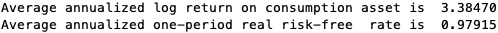
\includegraphics[scale = 0.75]{p4_output_1}

\bigskip

\item  What is the average conditional volatility of the stochastic discount factor? Decompose the volatility into components related to short-run, long-run, and volatility news.

\bigskip

\underline{Solution:}  The average conditional volatility of the stochastic discount factor and decomposition:

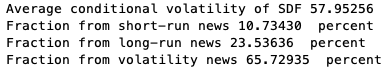
\includegraphics[scale = 0.75]{p4_output_2}

\bigskip

\item  Extend the code to solve for the term-structure of real rates, and the price-dividend ratio on the dividend-paying asset.

\bigskip

\underline{Solution:}  See \texttt{p4\_lrr.m}.

\pagebreak

\item  What are the model implications for the levels of the risk-free rates from 1 month to 5 years in maturity?

\bigskip

\underline{Solution:} The yield curve is below:

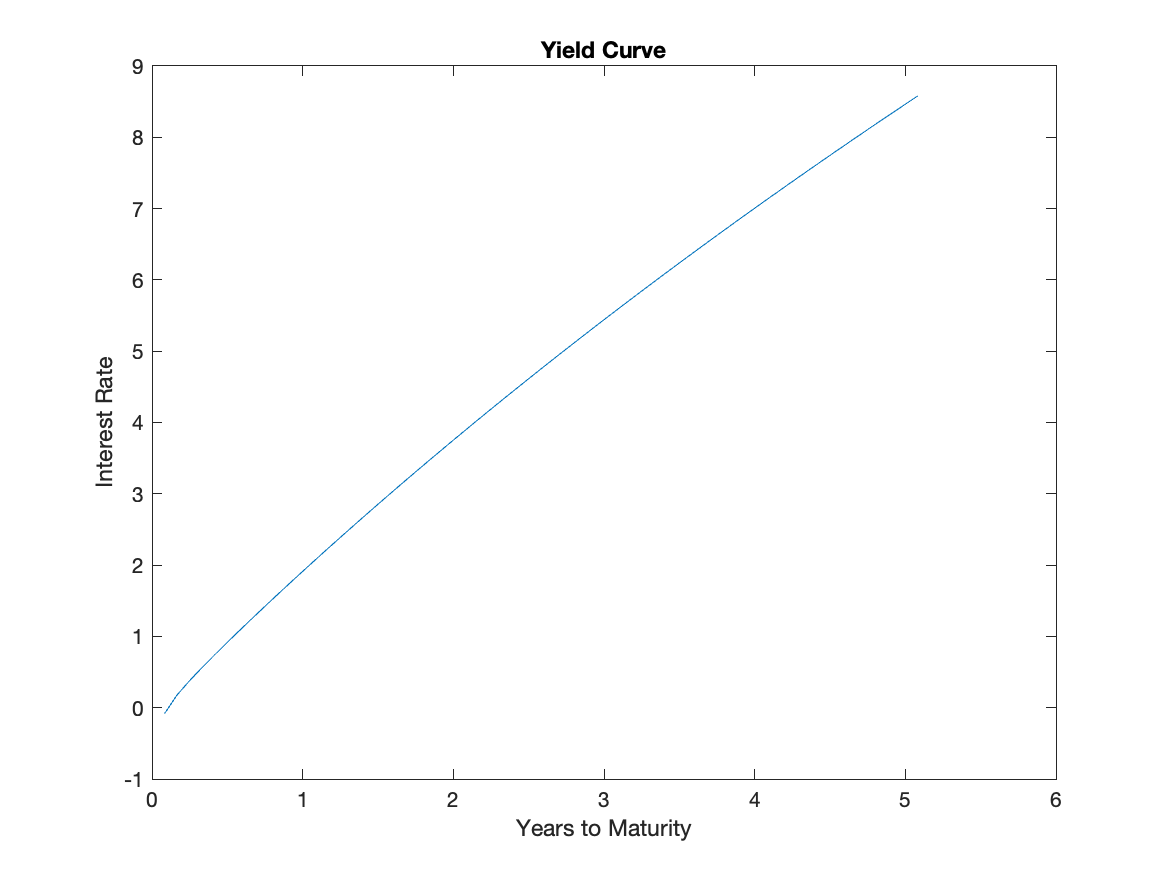
\includegraphics[scale = 0.75]{p4_output_4}

\bigskip

\item  What are the average log price-consumption and log price-dividend ratios? How does the market pd ratio compare to the data?

\bigskip

\underline{Solution:} The average log price-consumption and log price-dividend ratios are below along with market pd ratio from data:

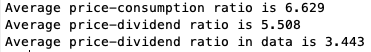
\includegraphics[scale = 0.75]{p4_output_5}

\bigskip

\item What is the average equity premium on consumption asset? on dividend-paying asset? Decompose the premia into components related to short-run, long-run and volatility risks.

\bigskip

\underline{Solution:}  The average equity premium on the consumption asset with decomposition is below:

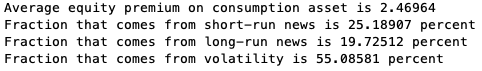
\includegraphics[scale = 0.75]{p4_output_6a}

\pagebreak

The average equity premium on the dividend-paying asset with decomposition is below:

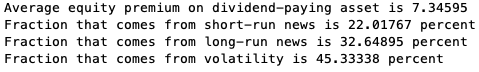
\includegraphics[scale = 0.75]{p4_output_6b}

\bigskip

\item  What is the volatility of equity returns and risk-free rates in the model?

\bigskip

\underline{Solution:} 

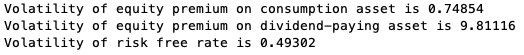
\includegraphics[scale = 0.75]{p4_output_7}

\bigskip

\item  Comment on the ability of the model to solve equity premium, risk-free rate, and return volatility puzzles.

\bigskip

\underline{Solution:}  This model seems to solve equity premium, risk-free rate, and return volatility puzzles pretty well.  In the data, the average stock return in excess of Treasury is about 5 percent, the risk-free rate is about 1 percent, and the volatility of equity returns is about 15-20 percent.  In the model, we have an average equity premium on the dividend-paying asset of about 7 percent, low risk-free rates with low volatility, and volatility of equity premium on dividend-paying asset of about 10 percent. We could play around with parameters to try to boost the volatility of the equity premium on the dividend-paying asset to get it higher.

\end{enumerate}

\end{document}